In diesem Kapitel werden alle Grundlagen erläutert, welche nötig sind um den Versuch durchführen zu können. 
\subsection{Die Lichtgeschwindkeit heute}
An der Internationalen Konferenz für Mass und Gewicht kurz ICPM wurde der Meter durch Festlegung des Zahlenwertes für die Lichgeschwindigkeit im Vakuum wie folgt neu definiert.

%%%%%%%%%%%%%%%%%%%%%%%%%%%%%%%%%%%%%%%%%%%%%%%%%%%%%%%%%%%%%%%%%%%%%%%%%%%%%
\begin{equation*}
c_{0} = 299'792'458 m/s
\label{eq:Lichtgeschwindigkeit}
\end{equation*}
%%%%%%%%%%%%%%%%%%%%%%%%%%%%%%%%%%%%%%%%%%%%%%%%%%%%%%%%%%%%%%%%%%%%%%%%%%%%%

Die Lichtgeschwindigkeit in einem Medium wiederrum erhält man mit Hilfe des gemessenen Brechungsindexes $n$ definiert in Formel \ref{eq:Formel_Brechungsindex}. In einem Gas, also zum Beispiel in der Luft, ist $n$ proportional zur Dichte und wird noch durch die Luftfeuchtigkeit leicht beeinflusst.

%%%%%%%%%%%%%%%%%%%%%%%%%%%%%%%%%%%%%%%%%%%%%%%%%%%%%%%%%%%%%%%%%%%%%%%%%%%%%
\begin{equation}
c=c_{0}/n
\label{eq:Formel_Brechungsindex}
\end{equation}
%%%%%%%%%%%%%%%%%%%%%%%%%%%%%%%%%%%%%%%%%%%%%%%%%%%%%%%%%%%%%%%%%%%%%%%%%%%%%

Um den Brechungsindex $n$ auszurechnen, kann Formel \ref{eq:Formel_Brechungsindex_in_der_Luft} angewandt werden, wobei diese jedoch noch nach $n$ umgeformt werden muss.

%%%%%%%%%%%%%%%%%%%%%%%%%%%%%%%%%%%%%%%%%%%%%%%%%%%%%%%%%%%%%%%%%%%%%%%%%%%%%
\begin{equation}
(n - 1) = (n_{n} - 1)\cdot\dfrac{p \cdot T_{n}}{p_{n} \cdot T}-(\beta - \dfrac{\gamma}{\lambda}_{0}) \cdot p_{w}
\label{eq:Formel_Brechungsindex_in_der_Luft}
\end{equation}
%%%%%%%%%%%%%%%%%%%%%%%%%%%%%%%%%%%%%%%%%%%%%%%%%%%%%%%%%%%%%%%%%%%%%%%%%%%%%

Die in Formel \ref{eq:Formel_Brechungsindex_in_der_Luft} enthaltenen Parameter sind unteranderem die gemessene Raumtemperatur $T$ in Kelvin, sowie der gemessene Luftdruck $p$. $\beta$ und $\gamma$ sind Wasserdampfkorrekturfaktoren, sowie $\lambda_{0}$ die Vakuum-Wellenlänge, welche unmerklich verschwinden von der Luftwellenlänge ist, weshalb diese verwendet wird.

%%%%%%%%%%%%%%%%%%%%%%%%%%%%%%%%%%%%%%%%%%%%%%%%%%%%%%%%%%%%%%%%%%%%%%%%%%%%%
\begin{equation*}
\beta = 4.292 \cdot 10^{-8} mbar^{-1},\;\gamma = 3.43 \cdot 10^{-2},\;\lambda_{0} = 632.8 nm (nm)^{2}mbar^{-1}
\label{eq:Faktor_Beta}
\end{equation*}
%%%%%%%%%%%%%%%%%%%%%%%%%%%%%%%%%%%%%%%%%%%%%%%%%%%%%%%%%%%%%%%%%%%%%%%%%%%%%

Mit Hilfe der nachfolgenden Abbildung \ref{fig:Wasserdampfsättigung und Normbrechungsindex}, können die restlichen Parameter bestimmt werden. So kann beispielsweise aus der Abbildung links die p-Sättigung gelesen werden, anhand der gemessenen Raumtermperatur oder in der rechten Abbildung auf Grund der vorgegebenen Wellenlänge der Normbrechnungsindex $(n_{n} - 1)$ herausgelesen werden. Die restlichen Parameter $T_{n}$ und $p_{n}$ sind ebenfalls in der rechten Abbildung ablesbar.

%%%%%%%%%%%%%%%%%%%%%%%%%%%%%%%%%%%%%%%%%%%%%%%%%%%%%%%%%%%%%%%%%%%%%%%%%%%%%
\begin{figure}[htb]
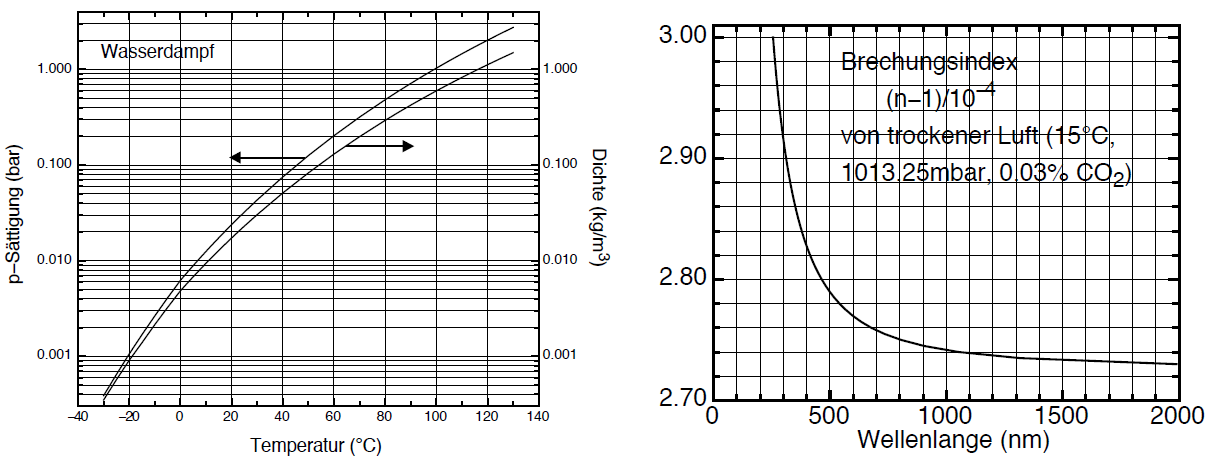
\includegraphics[width=\textwidth]{Brechungsindex_Luft_Grafik.png}
\caption{Wasserdampfsättigung und Normbrechungsindex}
\label{fig:Wasserdampfsättigung und Normbrechungsindex}
\end{figure}
%%%%%%%%%%%%%%%%%%%%%%%%%%%%%%%%%%%%%%%%%%%%%%%%%%%%%%%%%%%%%%%%%%%%%%%%%%%%%

%%%%%%%%%%%%%%%%%%%%%%%%%%%%%%%%%%%%%%%%%%%%%%%%%%%%%%%%%%%%%%%%%%%%%%%%%%%%%
\begin{equation}
p_{w} = \dfrac{Luftfeuchtigkeit}{100\%}\cdot p-Saettigung
\label{eq:Formel_Wasserdampfpartialdruck}
\end{equation}
%%%%%%%%%%%%%%%%%%%%%%%%%%%%%%%%%%%%%%%%%%%%%%%%%%%%%%%%%%%%%%%%%%%%%%%%%%%%%

Der Parameter $p_{w}$ wiederrum ist der Wasserdampfpartialdruck und wird separat mit Formel ausgerechnet, wobei der aus Abbildung \ref{fig:Wasserdampfsättigung und Normbrechungsindex} gelesene Wert verwendet wird, sowie die gemessene Luftfeuchtigkeit.


\subsection{Messung der Lichtgeschwindigkeit nach Michelson}
